\subsubsection{Convolutional Layer}
\label{sec:cnn-convolutional-layer}
The most important layer is the convolutional layer.
As the name suggests it performs a convolution with a filter matrix of arbitrary size on an input matrix of arbitrary size.
Let's say the input matrix is an image $\vec{X} \in \mathbb{R}^{m \times n}$.
The filter matrix $\vec{K} \in \mathbb{R}^{i \times j}$ contains $i \cdot j$ weights of the network.
The filter is now slid across the image and performs a dot product within its window.
\figref{fig:convolution} illustrates the following operation.
In reference to the figure, the kernel covers the four elements in the top right corner of the input image.
Hence, the dot product multiplication for this setup yields $5 \cdot 1+4 \cdot -1+1 \cdot -1+3 \cdot 1=3$.
This result is stored in a new matrix at its corresponding place.
In the end, this matrix will hold all values of the convolution operation.
After each calculation of the dot product, the filter matrix moves.
The corresponding step size is called stride.
A stride of 1 moves the filter one pixel or element, respectively.
There can be a different stride along the $x$-axis and $y$-axis.
When the filter has moved across the whole input, the resulting matrix is completely filled up like the one in the figure.
This resulting matrix is called a feature map because the convolution extracted features from its input.
\begin{figure}
	\centering
	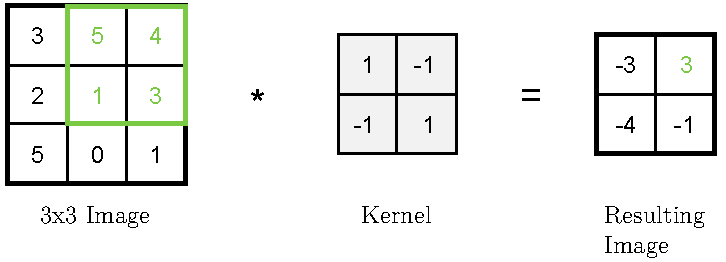
\includegraphics{images/convolution.pdf}
	\caption[Convolution of an image with a kernel]{Convolution of an image and a kernel. The $2 \times 2$ kernel is sled across the $3 \times 3$ image and performs a dot product multiplication within its window each time. Here, the kernel moves with a stride of 1, which results in the shown image on the right, the so-called feature map.}
	\label{fig:convolution}
\end{figure}
Doing this operation the feature map is always smaller than the input.
Sometimes this is not desirable, because this means a loss in information.
If multiple convolutions are performed, the feature map constantly shrinks until no feature can be extracted anymore or only rough ones.
Thus, a padding $p$ can be applied to the input.
This means surrounding the input with $p$ rounds of zeros like it is illustrated in \figref{fig:convolution-padding} with $p=1$.
The convolution operates like usual, just on a larger input.
\begin{figure}
	\centering
	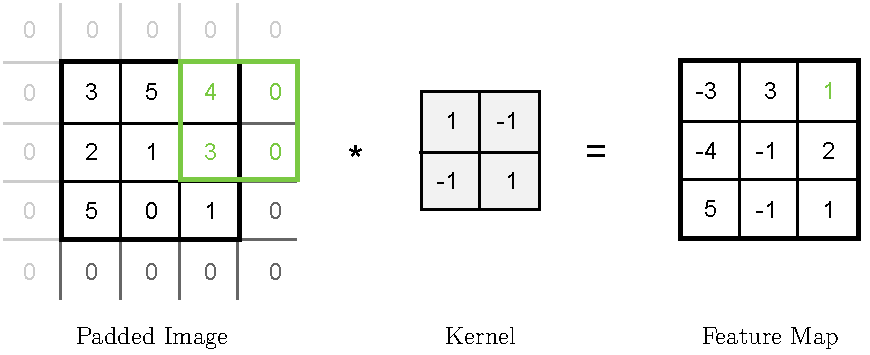
\includegraphics{images/convolution_padding.pdf}
	\caption[Convolution of a padded image with a kernel]{Convolution of a padded image with a $2 \times 2$ kernel. The $3 \times 3$ image is surrounded with zeros for inducing its size to the feature map. However, the convolution operates like usual, just on a larger input. If the amount of padding is odd, padding at the right and at the bottom is preferred.}
	\label{fig:convolution-padding}
\end{figure}
In practical terms, there are two common conventions for convolutions: valid and same.
The former defines that no padding is applied and therefore a kind of valid convolution is performed because only the real input is minded.
This means that the feature map has a size of $\vec{F} \in \mathbb{R}^{m-i+1 \times n-j+1}$.
The latter means, that the size of the feature map equals the one of the input.
How much padding $p$ needs to be applied can be calculated by comparing each matrix shapes and using
\begin{align}
	m &= m+2p-i+1 \\
	p &= \frac{i-1}{2}
\end{align}
as a general equation.
However, this only covers the padding height.
If the image or filter are not symmetrical, the padding along the width needs to be calculated as well by replacing $m$ with $n$ and $i$ with $j$.
Another remark is, that in computer vision filter sizes usually are odd.
There can be two reasons for this.
First, the filter has a center which helps to tell where exactly the filter points to.
Second, the padding $p$ is even.
Otherwise, it needs to be rounded up for a correct mathematical representation but only used on two sides of the image like it is shown in the figure with the help of transparency.
Only the padding at the right and at the bottom are taken into account for creating a filter matrix with the same shape of the original input.
For inputs with more than one channel, a convolution is performed almost identically.
But instead of a kernel with a depth of one, it is extended to a depth that matches the input.
Then a common dot product multiplication is calculated for every input channel with its corresponding filter channel.
This results in a matrix with the depth of the input and filter.
Finally, the resulting depth channels are summed up element-wise which results in a matrix with depth one.
For the case of an RGB image, that is an image with three channels representing the colors red, green and blue, a filter would have a depth of three and a final convolution result would always have a depth of one.
Usually, at the end of a convolutional layer, a bias addition is performed for simulating the neurobiological spike of a neuron.
This result is put into an activation function like the ones from \figref{fig:activation-functions} for introducing non-linearities into the network.
Both the methods and their purposes are analog to the ones known from multilayer perceptron networks.

The kernel in the figure would find top-left to bottom-right diagonal lines because those are the pixels weighted most.
Like this but with slightly larger kernels and different weights more complex features can be found.
It is also possible to perform multiple different convolutions on the same input for finding different features.
They are stored as a matrix, where the number of different features represents the depth of the feature map.
This whole process solves the limitation to a fixed position of features of the multilayer perceptrons architecture.
Even if, for example, a digit covers only have the image, all features are found, because the kernel is moved over the image and not single neurons or filters are responsible for single pixels.
Furthermore, because features are found by a moving filter, convolutional neural networks need way fewer weights and biases due to the possibility of reusing them.
The accuracy compared to multilayer perceptron networks is improved by concatenating several convolutions.
That means a convolution is performed on the feature map of an earlier convolution.
First, rough features like edges are found, and the deeper it gets into the network, the finer the features get.